\documentclass[11pt,a4paper]{article}

% --- Encoding and language ---
\usepackage[utf8]{inputenc}
\usepackage[T1]{fontenc}
\usepackage[english]{babel}

% --- Math and symbols ---
\usepackage{amsmath, amssymb, amsfonts}
\usepackage{siunitx}

% --- Page geometry ---
\usepackage[a4paper, margin=2.5cm]{geometry}

% --- Graphics and figures ---
\usepackage{graphicx}
\usepackage{subcaption}
\usepackage{float}
\graphicspath{{images/}}

% --- Tables ---
\usepackage{booktabs}
\usepackage{array}
\usepackage{multirow}

% --- Listings (code) ---
\usepackage{listings}
\usepackage{xcolor}

\definecolor{codegreen}{rgb}{0.0,0.5,0.0}
\definecolor{codegray}{rgb}{0.4,0.4,0.4}
\definecolor{codepurple}{rgb}{0.58,0,0.82}
\definecolor{codebg}{rgb}{0.96,0.96,0.96}

\lstdefinestyle{pythonstyle}{
    backgroundcolor=\color{codebg},
    commentstyle=\color{codegreen},
    keywordstyle=\color{blue}\bfseries,
    numberstyle=\tiny\color{codegray},
    stringstyle=\color{codepurple},
    basicstyle=\ttfamily\footnotesize,
    breakatwhitespace=false,
    breaklines=true,
    captionpos=b,
    keepspaces=true,
    numbers=left,
    numbersep=5pt,
    showspaces=false,
    showstringspaces=false,
    showtabs=false,
    tabsize=4,
    frame=single,
    rulecolor=\color{codegray},
    language=Python,
}
\lstset{style=pythonstyle}

% --- Hyperlinks ---
\usepackage[hidelinks]{hyperref}

% --- Caption tweaks ---
\usepackage[font=small,labelfont=bf]{caption}

% --- Section spacing ---
\usepackage{titlesec}
\titlespacing*{\section}{0pt}{1.2\baselineskip}{0.6\baselineskip}
\titlespacing*{\subsection}{0pt}{0.8\baselineskip}{0.4\baselineskip}

\begin{document}

% =====================================================================
\section{Task 1 -- Visualizing the floor plans}
% =====================================================================

The first task was to load and visualize the input data for a few floor plans to
get familiar with the dataset. Each building is represented by two NumPy arrays:
\texttt{<id>\_domain.npy} (a $512 \times 512$ grid with 5\,\textdegree C on
load-bearing walls, 25\,\textdegree C on inside walls and 0 elsewhere) and
\texttt{<id>\_interior.npy} (a boolean mask marking the cells that lie strictly
inside a room).

A small Python script
(\texttt{src/01-visualize-floorplans/visualize\_floorplans.py}) reads both files
for each building, builds a colour-coded RGB image of the domain (dark grey for
outside, blue for cold load-bearing walls, red for heated inside walls and white
for free interior cells) and plots it next to the binary interior mask. Some
representative results are shown in Figure~\ref{fig:task1-floorplans}.

\begin{figure}[H]
    \centering
    \begin{subfigure}[t]{0.48\textwidth}
        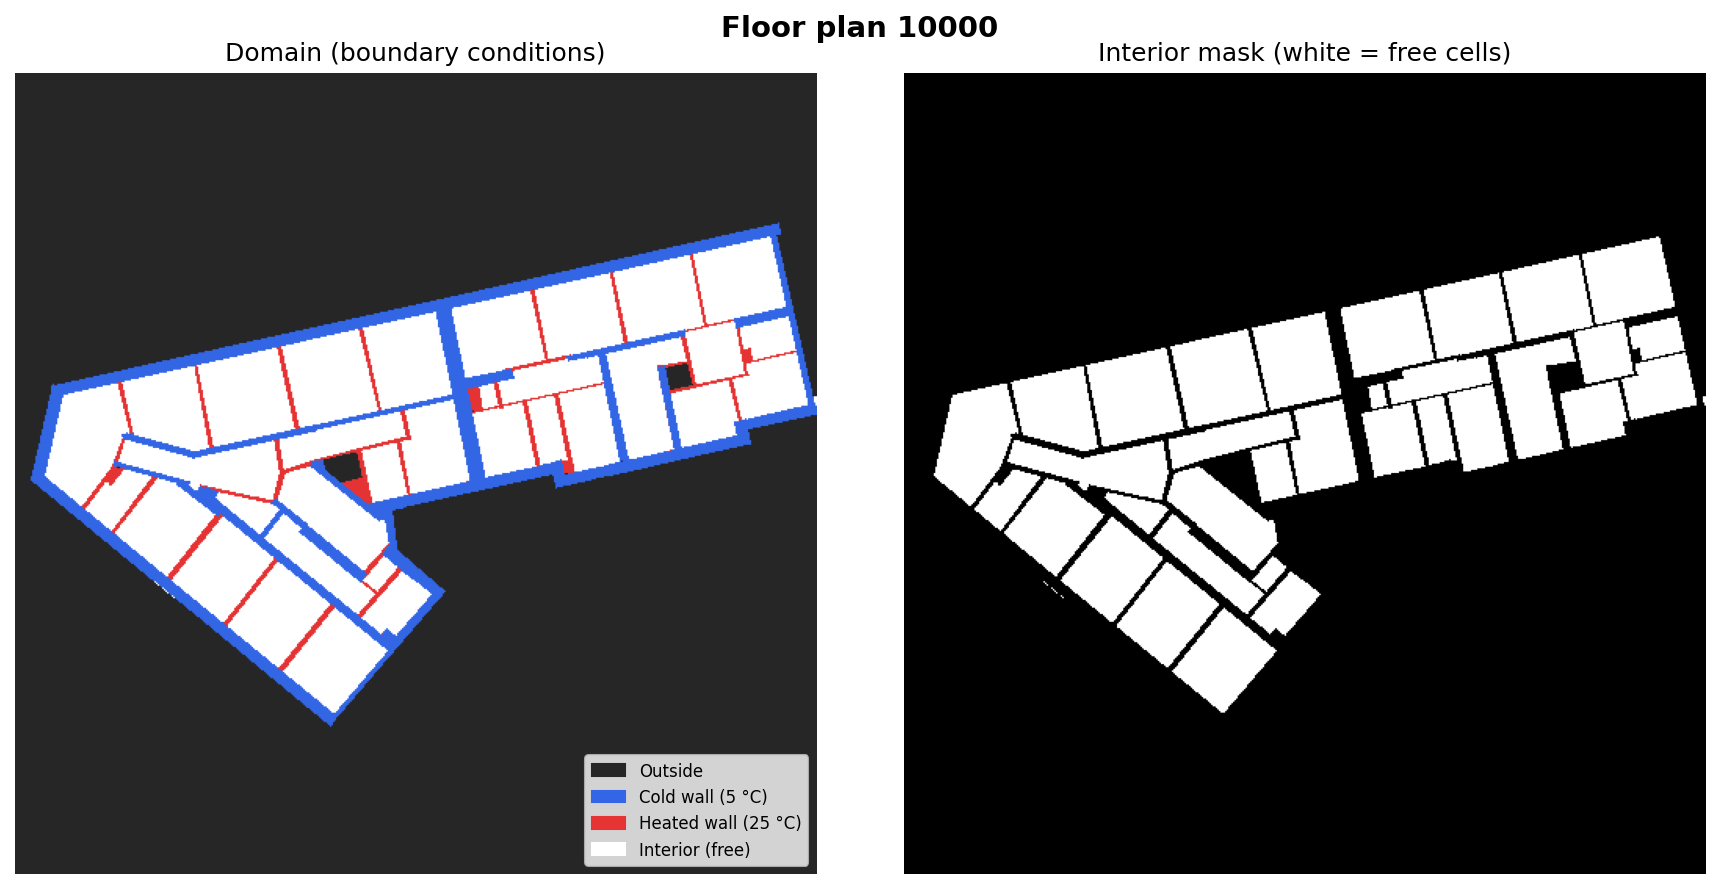
\includegraphics[width=\linewidth]{task1_floorplan_10000.png}
        \caption{Building 10000.}
    \end{subfigure}\hfill
    \begin{subfigure}[t]{0.48\textwidth}
        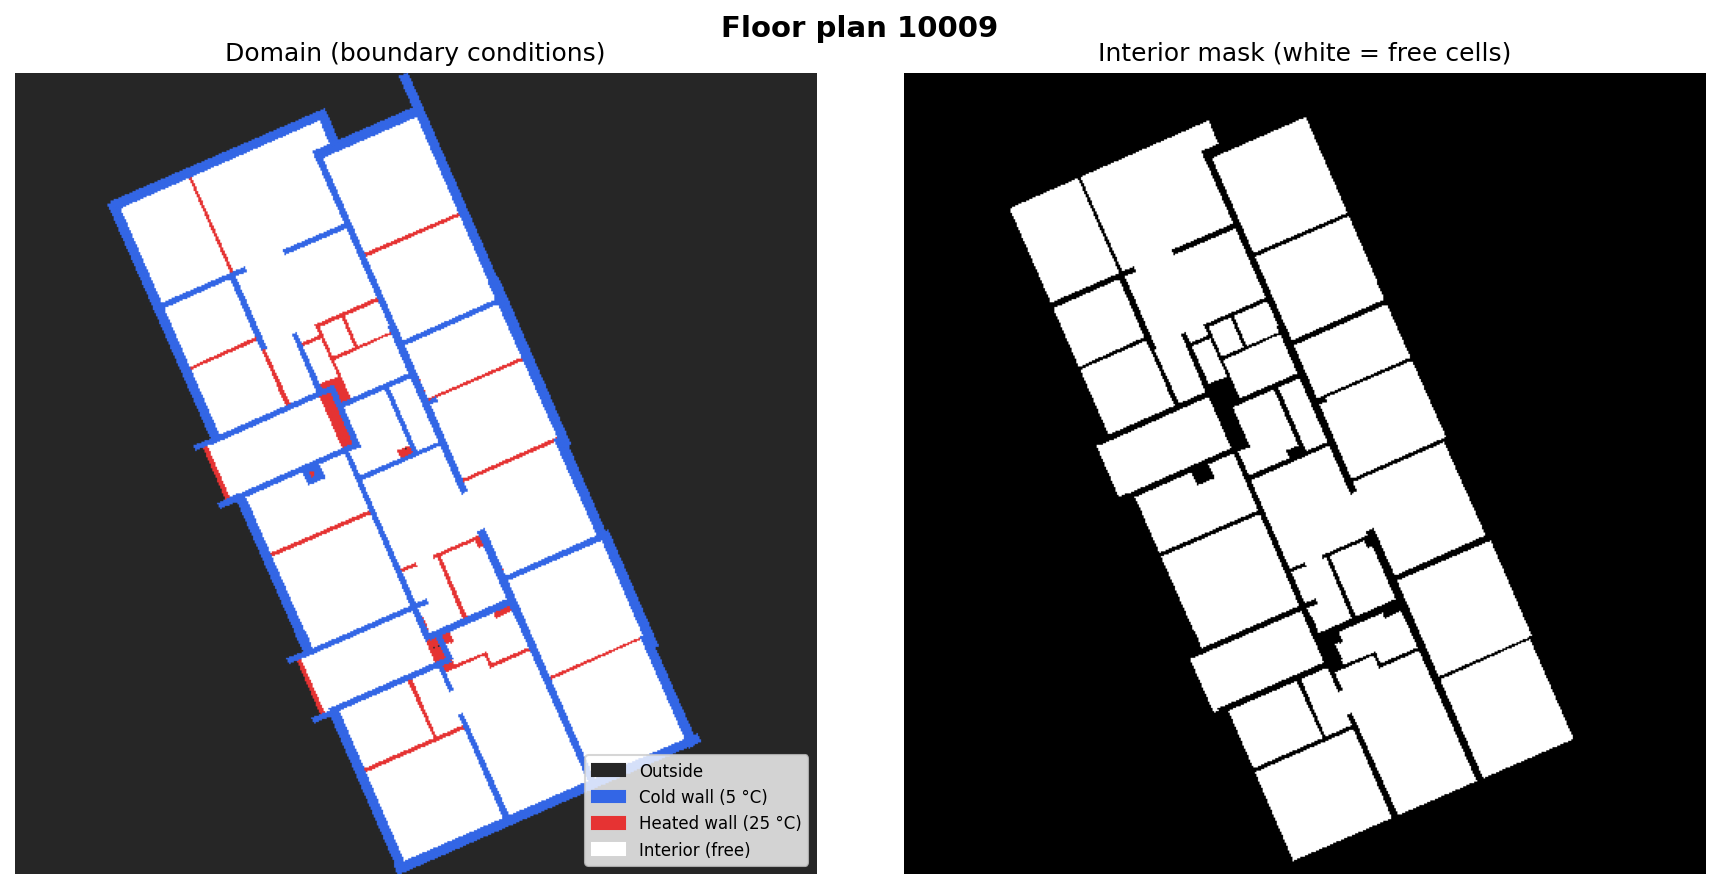
\includegraphics[width=\linewidth]{task1_floorplan_10009.png}
        \caption{Building 10009.}
    \end{subfigure}\\[1ex]
    \begin{subfigure}[t]{0.48\textwidth}
        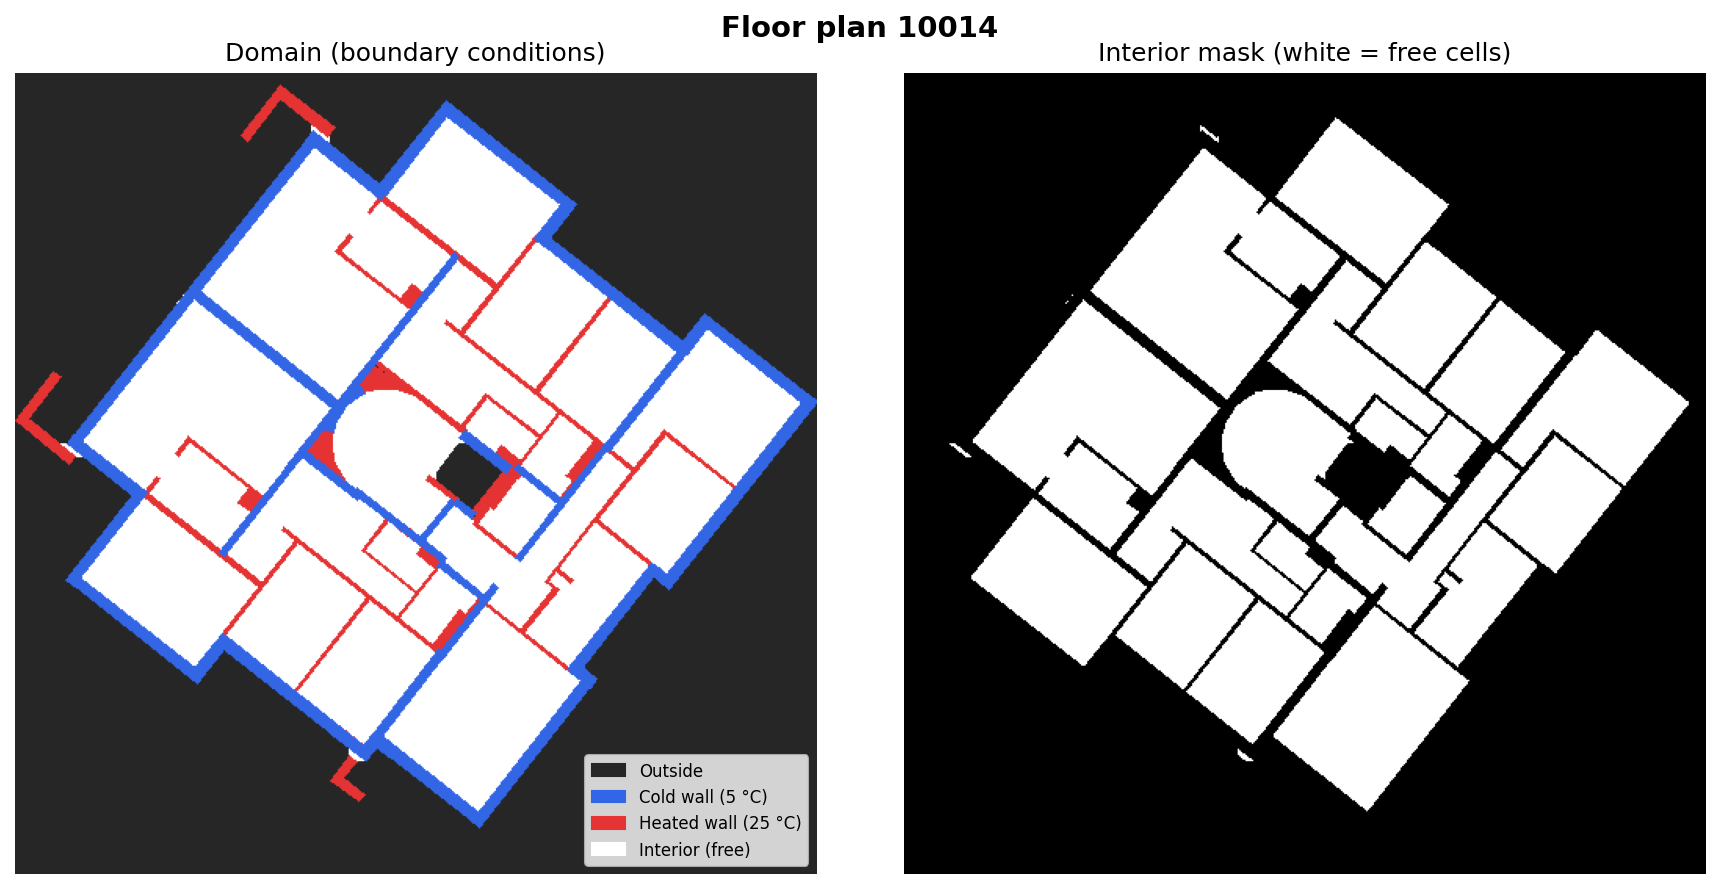
\includegraphics[width=\linewidth]{task1_floorplan_10014.png}
        \caption{Building 10014.}
    \end{subfigure}\hfill
    \begin{subfigure}[t]{0.48\textwidth}
        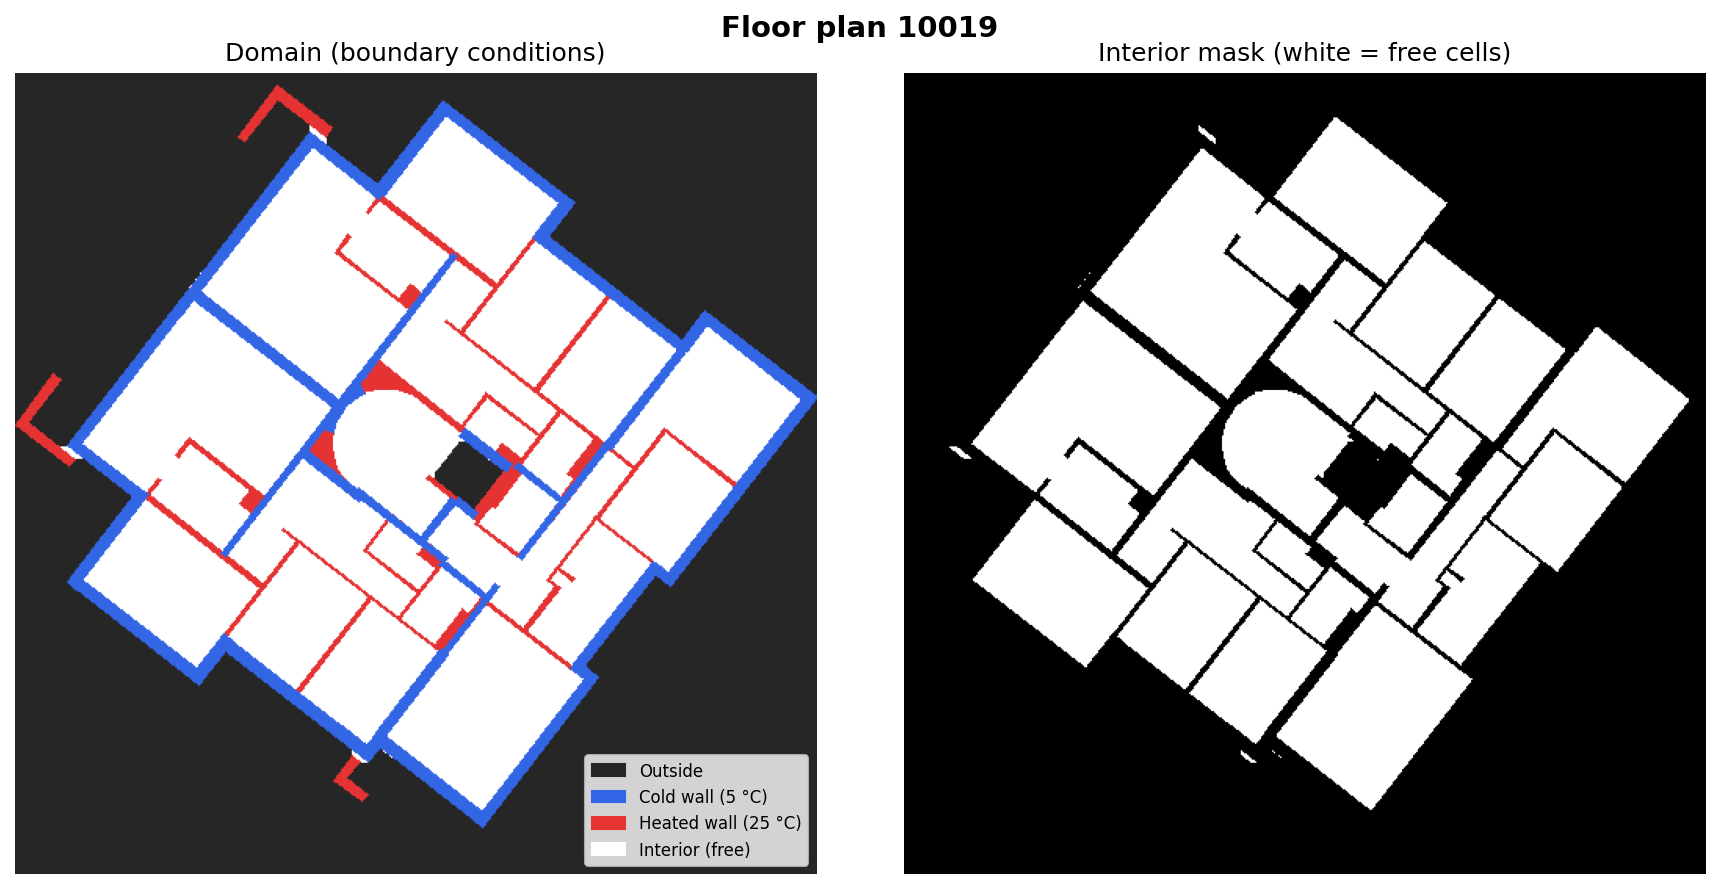
\includegraphics[width=\linewidth]{task1_floorplan_10019.png}
        \caption{Building 10019.}
    \end{subfigure}
    \caption{Example floor plans from the Modified Swiss Dwellings dataset. The
    left panel of each pair shows the colour-coded boundary conditions
    (red = inside walls at 25\,\textdegree C, blue = load-bearing walls at
    5\,\textdegree C, white = interior). The right panel shows the corresponding
    binary interior mask.}
    \label{fig:task1-floorplans}
\end{figure}

% =====================================================================
\section{Task 2 -- Reference benchmark}
% =====================================================================

The reference implementation in \texttt{simulate.py} was timed on a subset of
\(N = 10\) floor plans to estimate how long it would take to process the full
dataset of 4571 buildings. The benchmark was executed as an LSF batch job on the
DTU HPC \texttt{hpc} queue and repeated five times to obtain a reliable mean.

Each of the five repetitions ran in about \SI{86}{\second}, giving a mean of
\(86.255 \pm 0.886\)\,s for ten floor plans. This works out to
\(\approx \SI{8.625}{\second}\) per floor plan, so processing all 4571 floor
plans serially with the reference NumPy implementation would take roughly

\[
    8.625 \text{ s} \times 4571 \approx 39{,}426 \text{ s} \approx 657 \text{ min} \approx 10.95 \text{ h}.
\]

This is far too slow to be practical and motivates the optimisations performed
in the rest of the project. Table~\ref{tab:task2-timing} summarises the timing.

\begin{table}[H]
    \centering
    \begin{tabular}{lr}
        \toprule
        Quantity & Value \\
        \midrule
        Subset size & 10 floor plans \\
        Number of repeated runs & 5 \\
        Mean batch time & \SI{86.255}{\second} \\
        Standard deviation & \SI{0.886}{\second} \\
        Per-floor-plan time & \SI{8.625}{\second} \\
        Total floor plans available & 4571 \\
        Estimated time for full dataset & \SI{39426}{\second} ($\approx$ 10.95 h) \\
        \bottomrule
    \end{tabular}
    \caption{Reference (NumPy) timing on \(N = 10\) floor plans, run as an LSF
    batch job and averaged over five repetitions.}
    \label{tab:task2-timing}
\end{table}

% =====================================================================
\section{Task 3 -- Visualizing the simulation results}
% =====================================================================

Using the same reference solver, the steady-state temperature field was computed
for the first three floor plans of the subset and visualised next to the input
domain. Figure~\ref{fig:task3-simulations} shows three examples. As expected
from Laplace's equation, the temperature varies smoothly between the hot inside
walls (25\,\textdegree C) and the cold load-bearing walls (5\,\textdegree C),
with the warmest regions clustered around the inside walls and the coldest
regions near the outer load-bearing walls. The exact same image format is used
on the input domain (left) so that the boundary structure of each room can be
compared visually with the resulting temperature distribution (right).

\begin{figure}[H]
    \centering
    \begin{subfigure}[t]{0.48\textwidth}
        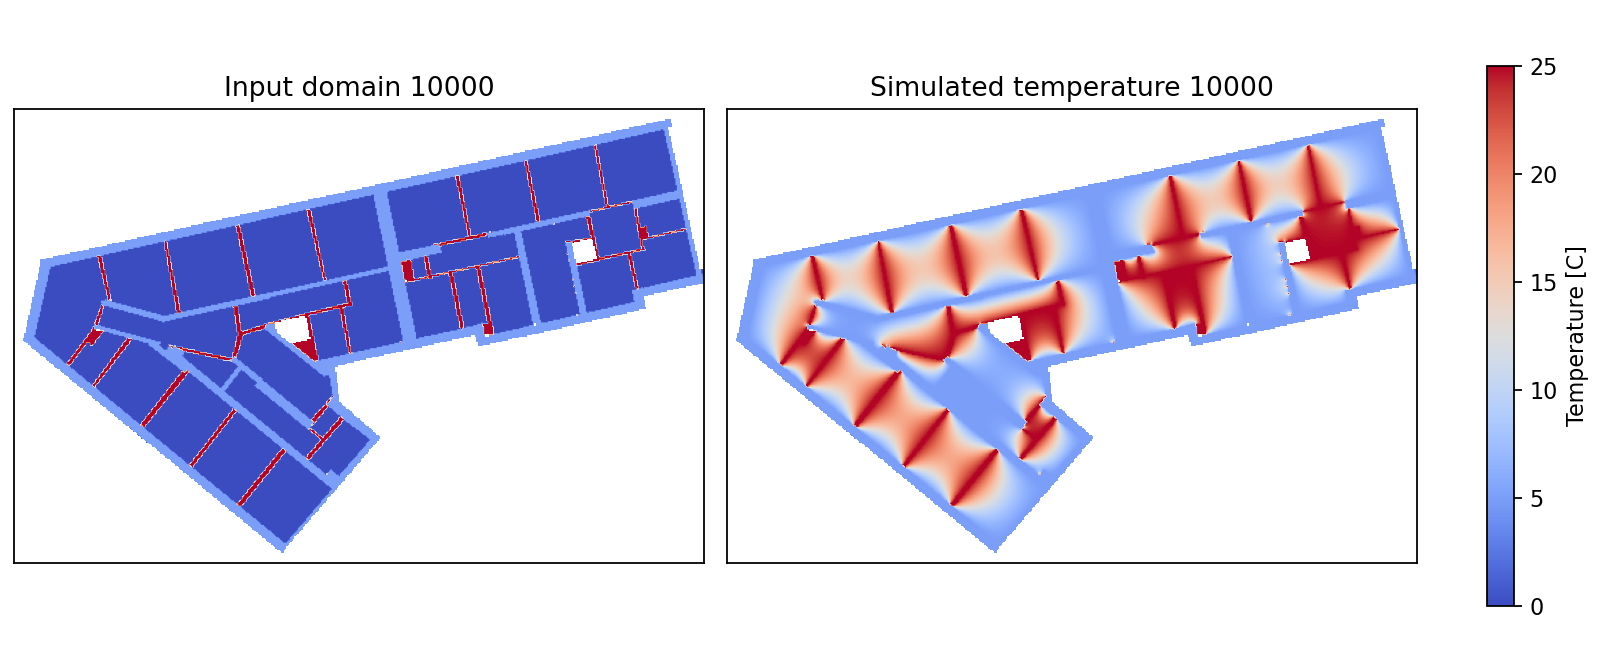
\includegraphics[width=\linewidth]{task3_simulation_10000.png}
        \caption{Building 10000.}
        \label{fig:task3-sim10000}
    \end{subfigure}\hfill
    \begin{subfigure}[t]{0.48\textwidth}
        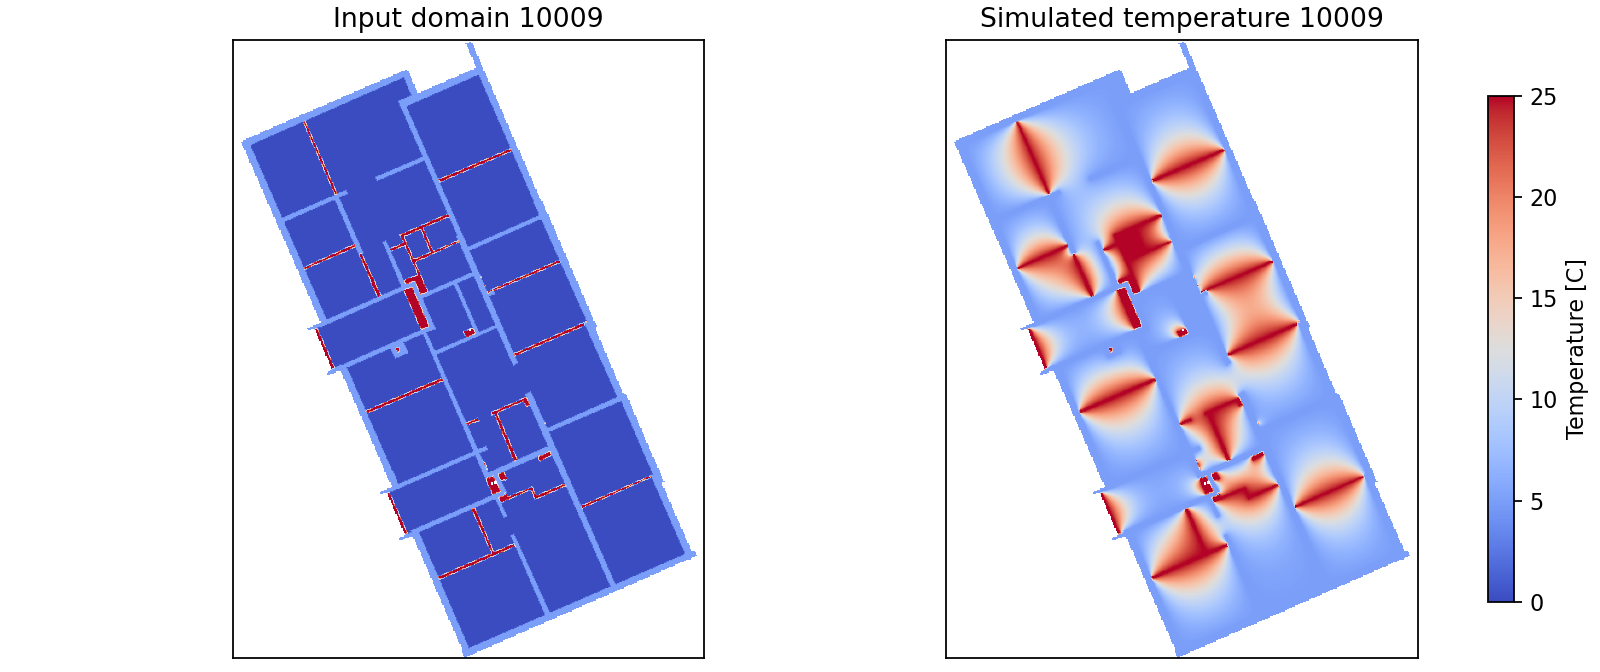
\includegraphics[width=\linewidth]{task3_simulation_10009.png}
        \caption{Building 10009.}
        \label{fig:task3-sim10009}
    \end{subfigure}\\[1ex]
    \begin{subfigure}[t]{0.48\textwidth}
        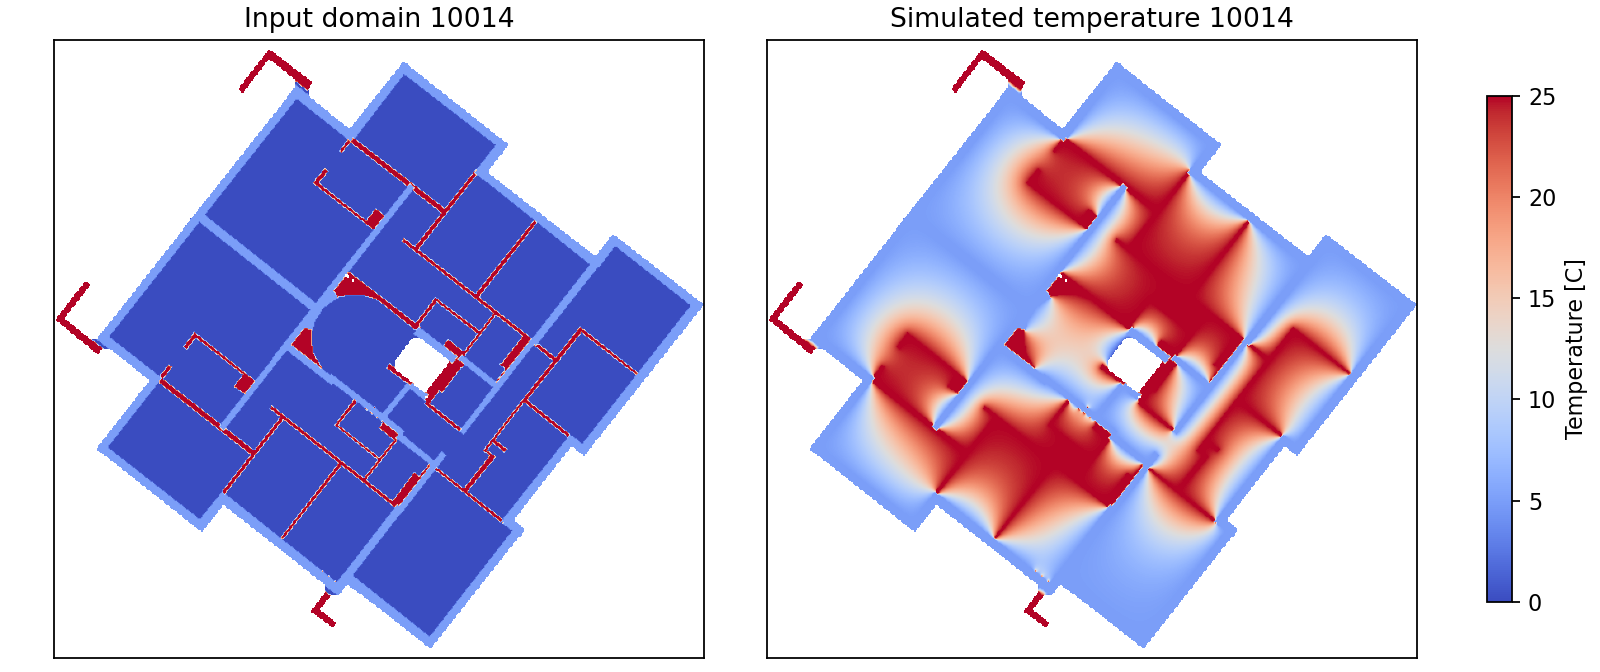
\includegraphics[width=\linewidth]{task3_simulation_10014.png}
        \caption{Building 10014.}
        \label{fig:task3-sim10014}
    \end{subfigure}
    \caption{Input domain (left) versus simulated steady-state temperature
    (right) after the Jacobi solver has converged, for three example
    buildings.}
    \label{fig:task3-simulations}
\end{figure}

\noindent The summary statistics for these three buildings (mean temperature,
standard deviation, percentage of area above 18\,\textdegree C and below
15\,\textdegree C) will be revisited for the full dataset in Task~12.

% =====================================================================
\section{Task 4 -- Profiling the reference \texttt{jacobi} function}
% =====================================================================

The reference \texttt{jacobi} function was profiled with \texttt{kernprof}
(line\_profiler) on a single floor plan, producing
\texttt{outputs/04-profiling/simulate.py.lprof}. The function executes 3602
Jacobi iterations before converging, so per-line totals are dominated by the
loop body. Table~\ref{tab:task4-profiling} reports the cumulative time spent on
each significant line, expressed in seconds and as a percentage of total
\texttt{jacobi} time (\SI{5.30}{\second}).

\begin{table}[H]
    \centering
    \begin{tabular}{lrr}
        \toprule
        Code section (per iteration) & Total time (s) & \% of total \\
        \midrule
        \texttt{u\_new = 0.25 * (u[1:-1, :-2] + u[1:-1, 2:] + \ldots)} & 3.246 & 61.2\% \\
        \texttt{delta = np.abs(...).max()} (convergence check) & 0.897 & 16.9\% \\
        \texttt{u[1:-1, 1:-1][interior\_mask] = u\_new\_interior} & 0.617 & 11.6\% \\
        \texttt{u\_new\_interior = u\_new[interior\_mask]} & 0.539 & 10.2\% \\
        \texttt{if delta < atol: break} & 0.003 & 0.05\% \\
        Pre-loop \texttt{u = np.copy(u)} & 0.002 & 0.04\% \\
        \bottomrule
    \end{tabular}
    \caption{Line-profiler breakdown of the reference \texttt{jacobi} function
    for one floor plan (3602 iterations, total \SI{5.30}{\second}).}
    \label{tab:task4-profiling}
\end{table}

\paragraph{Interpretation.} The hot path is clearly the five-point stencil
update (\(\approx 61\%\)), which builds the full \texttt{u\_new} array on every
iteration. The convergence check together with the two masked indexing
operations consumes another \(\approx 39\%\). All four costly lines run on every
one of the 3602 iterations, while the early-stopping branch and the initial
copy are essentially free. This profile motivates Tasks~7--10: replacing the
NumPy stencil with a JIT-compiled or GPU kernel removes the array-allocation
overhead, while batching the convergence check (Task~10) eliminates the only
serialising piece of work in the loop body.

% =====================================================================
\section{Task 5 -- Static scheduling}
% =====================================================================

A new entry point, \texttt{simulate\_static\_scheduling.py}, parallelises the
work across floor plans using Python's \texttt{multiprocessing.Pool}. Each
worker independently loads its assigned buildings from disk, runs the
Jacobi solver and returns the summary statistics, so no large NumPy arrays
have to be pickled across process boundaries. Static scheduling is implemented
by passing \texttt{chunksize = $\lceil N / P \rceil$} to \texttt{pool.map},
which gives every worker a contiguous block of floor plans.

The benchmark was run on \(N = 100\) floor plans on the DTU \texttt{hpc} queue
using a single node with up to 64 cores. The results are shown in
Table~\ref{tab:task5-timings} and Figure~\ref{fig:task5-speedup}.

\begin{table}[H]
    \centering
    \begin{tabular}{rrr}
        \toprule
        Workers \(P\) & Time \([s]\) & Speed-up \(S(P)\) \\
        \midrule
        1  & 763.63 & 1.00 \\
        2  & 419.01 & 1.82 \\
        4  & 213.95 & 3.57 \\
        8  & 144.47 & 5.29 \\
        16 & 79.81  & 9.57 \\
        32 & 54.40  & 14.04 \\
        64 & 43.20  & 17.68 \\
        \bottomrule
    \end{tabular}
    \caption{Static scheduling timing and speed-up on 100 floor plans.}
    \label{tab:task5-timings}
\end{table}

\begin{figure}[H]
    \centering
    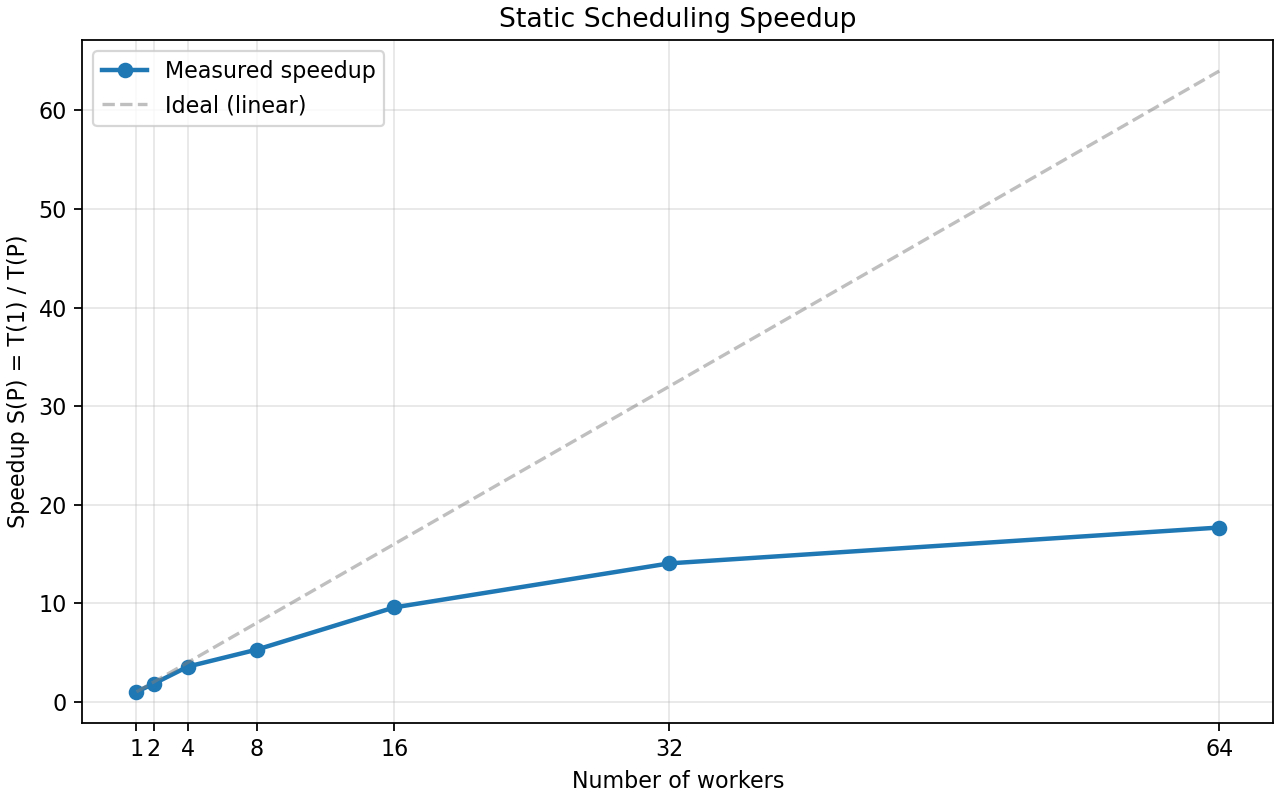
\includegraphics[width=0.7\linewidth]{task5_speedup_static.png}
    \caption{Measured speed-up of the static scheduling implementation versus
    the ideal linear scaling. The curve is sub-linear due to the serial
    fraction of the computation and to load imbalance across floor plans
    with different convergence times.}
    \label{fig:task5-speedup}
\end{figure}

\subsection*{5b) Parallel fraction (Amdahl's law)}

Amdahl's law states
\[
    S(P) = \frac{1}{(1-f) + f/P}
\]
which can be inverted to estimate the parallel fraction \(f\) from a measured
speed-up:
\[
    f = \frac{1 - 1/S}{1 - 1/P}.
\]
Substituting the best-measured speed-up \(S = 17.68\) at \(P = 64\) gives
\[
    f = \frac{1 - 1/17.68}{1 - 1/64} = \frac{0.9434}{0.9844} \approx 0.958.
\]
Approximately \(\mathbf{95.8\%}\) of the computation is parallelisable.

\subsection*{5c) Theoretical maximum speed-up}

\[
    S_\text{max} = \frac{1}{1 - f} = \frac{1}{1 - 0.958} \approx 24.0.
\]

The achieved speed-up of 17.68\(\times\) at \(P = 64\) corresponds to about
\(\mathbf{73.5\%}\) of the theoretical maximum. Diminishing returns are clearly
visible past \(P = 16\): doubling from 32 to 64 workers only improves the
speed-up from 14.04\(\times\) to 17.68\(\times\) (a \(1.26\times\) gain),
indicating that the serial overhead and load imbalance dominate at higher worker
counts.

\subsection*{5d) Estimate for the full dataset}

Using the fastest configuration (\(P = 64\), \SI{43.20}{\second} for 100 floor
plans) the per-floor-plan time is \SI{0.432}{\second}, so the full dataset of
4571 buildings would take
\[
    0.432 \text{ s} \times 4571 \approx 1975 \text{ s} \approx 32.9 \text{ min}.
\]

% =====================================================================
\section{Task 6 -- Dynamic scheduling}
% =====================================================================

The same parallel benchmark was repeated with dynamic scheduling
(\texttt{chunksize = 1}), so that whenever a worker finishes a floor plan it
immediately picks up the next available one. The remaining setup is identical
to Task~5.

\subsection*{6a) Did it get faster?}

Table~\ref{tab:task6-comparison} compares the wall-clock times of static and
dynamic scheduling for every worker count. Dynamic scheduling is consistently
faster, with the largest absolute gain at \(P = 8\) (\SI{43.85}{\second} or
roughly 30\% faster). The improvement at \(P = 1\) is small and within
run-to-run variance, since both configurations execute sequentially.

\begin{table}[H]
    \centering
    \begin{tabular}{rrrr}
        \toprule
        Workers \(P\) & Static \([s]\) & Dynamic \([s]\) & Difference \\
        \midrule
        1  & 763.63 & 734.73 & baseline \\
        2  & 419.01 & 367.17 & 51.84 s faster \\
        4  & 213.95 & 191.69 & 22.27 s faster \\
        8  & 144.47 & 100.62 & 43.85 s faster \\
        16 & 79.81  & 58.50  & 21.31 s faster \\
        32 & 54.40  & 38.82  & 15.58 s faster \\
        64 & 43.20  & 37.40  & 5.80 s faster \\
        \bottomrule
    \end{tabular}
    \caption{Wall-clock time per worker count for static vs dynamic scheduling
    on 100 floor plans.}
    \label{tab:task6-comparison}
\end{table}

The reason dynamic scheduling wins is \textbf{load balancing}: different floor
plans require different numbers of Jacobi iterations to converge, so a static
block can be dominated by a single slow building while other workers sit idle.
With \texttt{chunksize = 1} the queue keeps every worker busy until the very
last building has been dispatched.

\subsection*{6b) Did the speed-up improve?}

\begin{table}[H]
    \centering
    \begin{tabular}{rrr}
        \toprule
        Workers \(P\) & Static speed-up & Dynamic speed-up \\
        \midrule
        1  & 1.00  & 1.00 \\
        2  & 1.82  & 2.00 \\
        4  & 3.57  & 3.83 \\
        8  & 5.29  & 7.30 \\
        16 & 9.57  & 12.56 \\
        32 & 14.04 & 18.93 \\
        64 & 17.68 & 19.65 \\
        \bottomrule
    \end{tabular}
    \caption{Speed-up of static vs dynamic scheduling.}
    \label{tab:task6-speedups}
\end{table}

\begin{figure}[H]
    \centering
    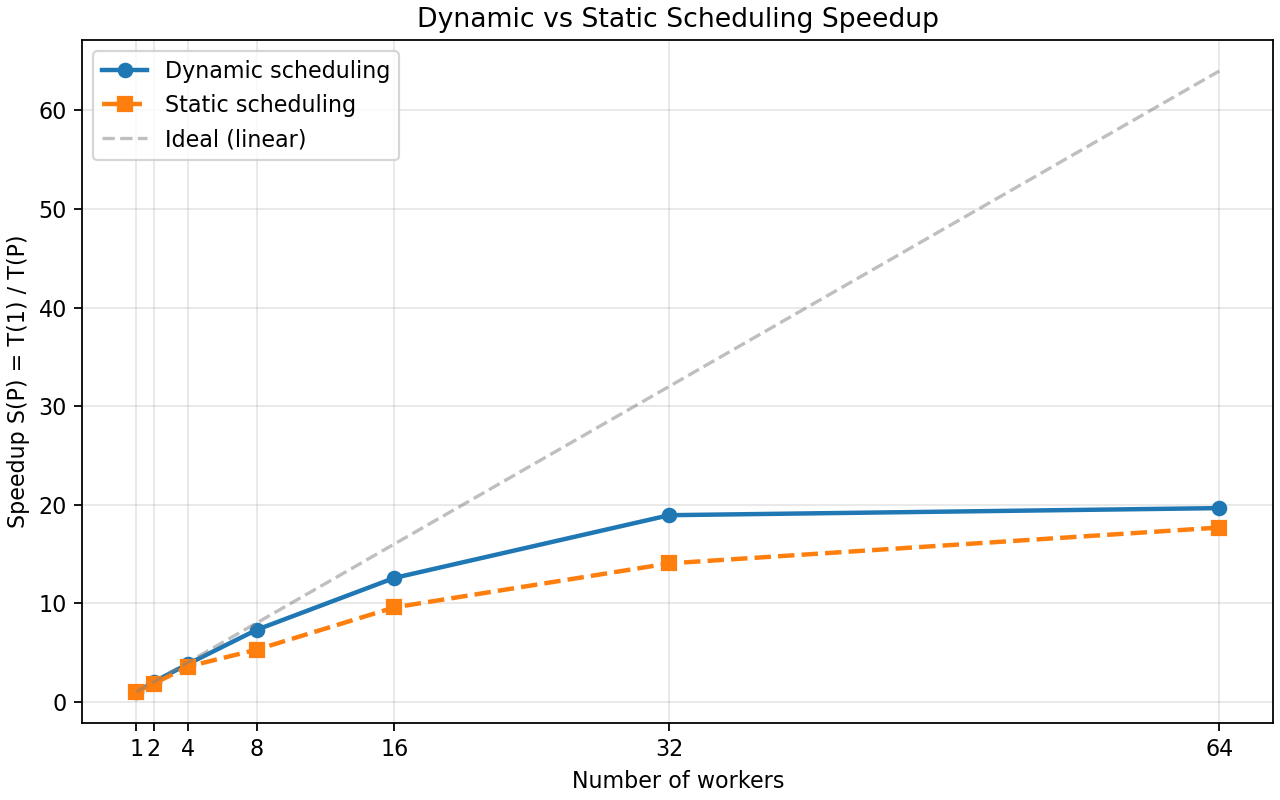
\includegraphics[width=0.7\linewidth]{task6_speedup_dynamic_vs_static.png}
    \caption{Speed-up curves for dynamic and static scheduling versus the ideal
    linear scaling. Dynamic scheduling is closer to linear at every worker
    count and the gap to static widens as more workers are added.}
    \label{fig:task6-speedup}
\end{figure}

The speed-up improved across the board, and the gap widens with more workers.
At \(P = 32\) dynamic reaches \(18.93\times\) versus static's
\(14.04\times\), a substantial gain. At \(P = 64\) dynamic reaches
\(19.65\times\) versus \(17.68\times\), but the gain flattens, indicating that
the remaining bottleneck is no longer load imbalance but the unavoidable
serial overhead (process startup, I/O, result aggregation).

% =====================================================================
\section{Task 7 -- Numba JIT on the CPU}
% =====================================================================

In Task~7 the \texttt{jacobi} function was rewritten as a Numba JIT-compiled
kernel that runs on a single CPU core (\texttt{simulate\_numba\_jit\_cpu.py}).
The pure-Python solver uses two explicit nested loops (outer over rows
\texttt{i}, inner over columns \texttt{j}) and applies the five-point stencil
directly:

\begin{lstlisting}
@numba.njit
def jacobi_numba(u, interior_mask, max_iter, atol=1e-6):
    u = u.copy()
    u_new = u.copy()
    for _ in range(max_iter):
        delta = 0.0
        for i in range(512):
            for j in range(512):
                if interior_mask[i, j]:
                    val = 0.25 * (u[i+1, j] + u[i+1, j+2]
                                  + u[i, j+1] + u[i+2, j+1])
                    d = val - u[i+1, j+1]
                    if d < 0.0:
                        d = -d
                    if d > delta:
                        delta = d
                    u_new[i+1, j+1] = val
        u, u_new = u_new, u
        if delta < atol:
            break
    return u
\end{lstlisting}

\subsection*{7a) Timing and comparison to the reference}

The benchmark was run on \(N = 10\) floor plans on the DTU \texttt{hpc} queue
(single core). Results are shown in Table~\ref{tab:task7-timing} and
Figure~\ref{fig:task7-timing}.

\begin{table}[H]
    \centering
    \begin{tabular}{lr}
        \toprule
        Metric & Value \\
        \midrule
        Wall time (incl.\ JIT compile) & \SI{38.901}{\second} \\
        Internal time (post-warmup)    & \SI{36.432}{\second} \\
        Per-floor-plan (internal)      & \SI{3.643}{\second} \\
        Reference per-floor-plan (NumPy, Task~2) & \SI{8.625}{\second} \\
        \textbf{Speed-up vs reference} & \(\mathbf{2.37\times}\) \\
        \bottomrule
    \end{tabular}
    \caption{Numba JIT CPU timing on \(N = 10\) floor plans.}
    \label{tab:task7-timing}
\end{table}

\begin{figure}[H]
    \centering
    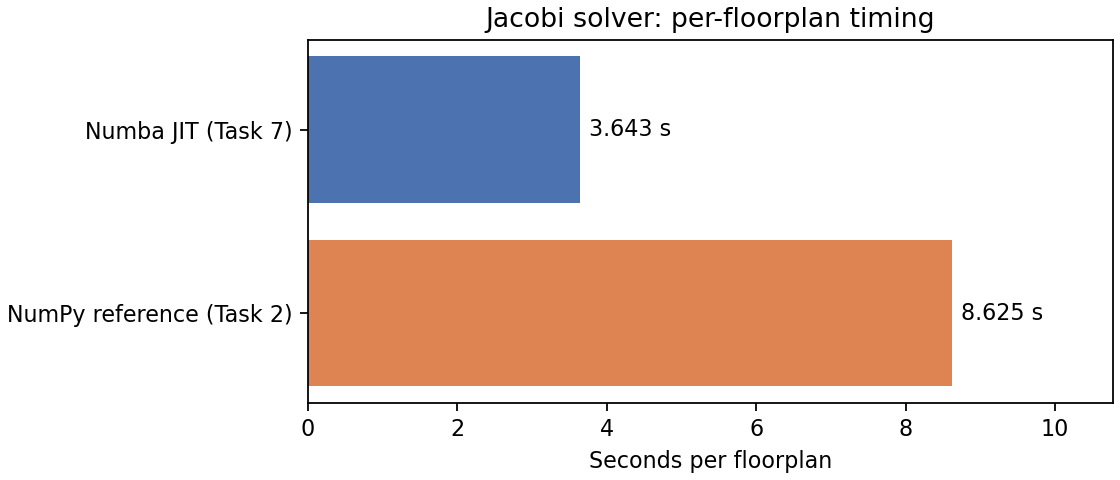
\includegraphics[width=0.7\linewidth]{task7_timing_comparison.png}
    \caption{Per-floor-plan timing of the Numba JIT CPU solver versus the
    NumPy reference.}
    \label{fig:task7-timing}
\end{figure}

The Numba solution is \(2.37\times\) faster than the reference. The one-time
JIT compilation (\(\sim\!2.5\) s, the difference between wall time and internal
time) is amortised over the rest of the run.

\subsection*{7b) Function explanation and cache access pattern}

The \texttt{@numba.njit} decorator compiles the function to native machine code
and removes both the Python interpreter overhead and the temporary-array
overhead of the NumPy stencil. Because NumPy arrays are stored in row-major
(C-contiguous) order, iterating with \texttt{i} as the outer loop and \texttt{j}
as the inner loop walks each row left-to-right one element at a time. All four
stencil neighbours (\texttt{u[i+1, j]}, \texttt{u[i+1, j+2]}, \texttt{u[i, j+1]}
and \texttt{u[i+2, j+1]}) come from rows \texttt{i}, \texttt{i+1} and
\texttt{i+2}, which fit comfortably together in L2/L3 cache. Each inner-loop
step advances one element along these three rows, so the access pattern is
cache-line friendly with no strided or random accesses.

The convergence check is also kept inside the JIT-compiled region: a plain
scalar \texttt{delta} is updated in place, avoiding any NumPy reduction call
that would force Numba to drop back to the Python interpreter.

\subsection*{7c) Estimate for the full dataset}

\[
    3.643 \text{ s} \times 4571 \approx 16{,}653 \text{ s} \approx 277.6 \text{ min} \approx 4.6 \text{ h}.
\]

This is roughly \(2.4\times\) faster than the NumPy reference estimate, but
still impractical on a single core. Multi-core parallelism (Tasks 5--6) or GPU
acceleration (Tasks 8--10) is needed to bring the full dataset within reach.

% =====================================================================
\section{Task 8 -- Custom Numba CUDA kernel}
% =====================================================================

\subsection*{8a) Kernel and helper structure}

Task 8 implements a custom CUDA kernel with Numba
(\texttt{simulate\_numba\_cuda.py}). The kernel performs \emph{a single} Jacobi
iteration; the Python helper repeatedly launches it for a fixed number of
iterations, with no early-stopping criterion.

\begin{lstlisting}
@cuda.jit
def _jacobi_kernel(u, u_new, interior_mask_u8):
    i, j = cuda.grid(2)
    if i < 512 and j < 512:
        if interior_mask_u8[i, j] != 0:
            u_new[i+1, j+1] = 0.25 * (u[i+1, j] + u[i+1, j+2]
                                      + u[i, j+1] + u[i+2, j+1])
\end{lstlisting}

The launch configuration uses 16$\times$16-thread blocks covering the full
\(512 \times 512\) interior grid (256 threads per block, a common choice that
keeps each block small enough for the streaming multiprocessors to schedule
many concurrently). Each thread updates exactly one cell; non-interior cells
are never written so the fixed boundary conditions are preserved automatically. The interior mask is
stored as \texttt{uint8} rather than \texttt{bool} to avoid device-array
instabilities seen on some CUDA driver versions.

The Python helper \texttt{jacobi\_numba\_cuda} owns two device buffers
(\texttt{d\_u}, \texttt{d\_u\_new}) and double-buffers them: after each kernel
launch the references are swapped so the freshly written values become the read
source for the next iteration. Both buffers are initialised from the input
\texttt{u}, so the ghost rows used by the stencil are present from the start.
The kernel boundary itself acts as a global barrier between iterations: no
intra-kernel synchronisation is needed because each thread writes only to its
own output cell.

\subsection*{8b) Timing and comparison to the reference}

The benchmark was run twice on \(N = 10\) floor plans on a DTU A100 GPU.
Results are shown in Table~\ref{tab:task8-timing}.

\begin{table}[H]
    \centering
    \begin{tabular}{lrr}
        \toprule
        Metric & Run 1 & Run 2 \\
        \midrule
        Wall time (incl.\ CUDA JIT) & \SI{9.751}{\second} & \SI{9.604}{\second} \\
        Internal time (post-warmup) & \SI{8.354}{\second} & \SI{8.214}{\second} \\
        Per-floor-plan (internal)   & \SI{0.835}{\second} & \SI{0.821}{\second} \\
        Reference per-floor-plan    & \multicolumn{2}{c}{\SI{8.625}{\second}} \\
        \textbf{Speed-up vs reference} & \(\mathbf{10.3\times}\) & \(\mathbf{10.5\times}\) \\
        \bottomrule
    \end{tabular}
    \caption{Numba CUDA timing on \(N = 10\) floor plans (A100 GPU).}
    \label{tab:task8-timing}
\end{table}

\begin{figure}[H]
    \centering
    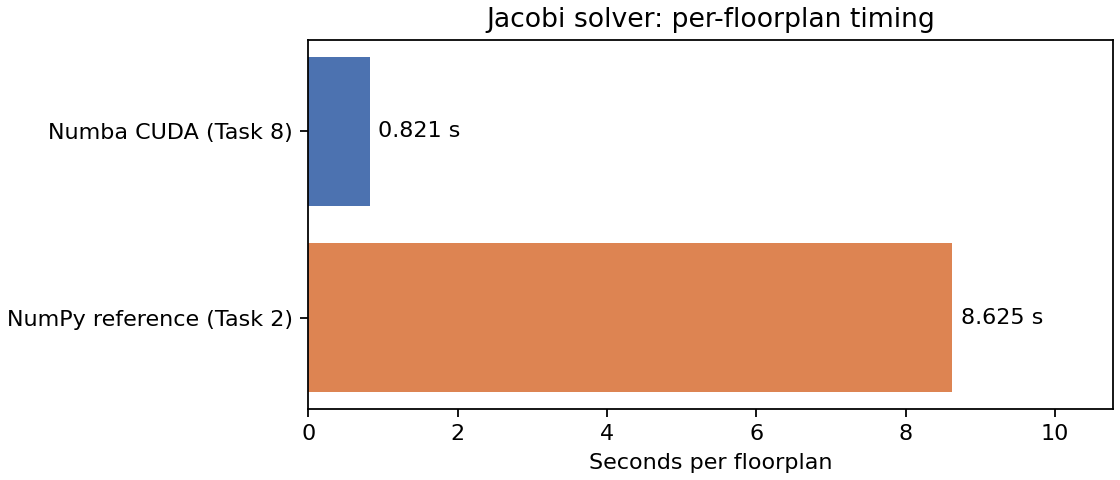
\includegraphics[width=0.7\linewidth]{task8_timing_comparison.png}
    \caption{Per-floor-plan timing of the Numba CUDA solver versus the
    NumPy reference.}
    \label{fig:task8-timing}
\end{figure}

The two runs agree to within \(\approx 1.7\%\), confirming that the timing is
reliable. The Numba CUDA kernel is roughly \(\mathbf{10.4\times}\) faster than
the NumPy reference, and the JIT-compilation overhead (\(\approx 1.4\) s) is
small.

\subsection*{8c) Estimate for the full dataset}

\[
    0.821 \text{ s} \times 4571 \approx 3{,}754 \text{ s} \approx 62.6 \text{ min} \approx 1.0 \text{ h}.
\]

This is a \(4.4\times\) improvement over the Numba CPU solution from Task~7
and makes processing the full dataset in a single GPU job practical.

% =====================================================================
\section{Task 9 -- CuPy reference port}
% =====================================================================

\subsection*{9a) Timing and comparison to the reference}

In Task~9 the reference solver was ported to CuPy
(\texttt{simulate\_cupy.py}). The implementation mirrors the NumPy reference
almost line-for-line, with \texttt{np} replaced by \texttt{cp}, but
the convergence check still runs every iteration. Results on \(N = 10\) floor
plans on the A100 are shown in Table~\ref{tab:task9-timing}.

\begin{table}[H]
    \centering
    \begin{tabular}{lr}
        \toprule
        Metric & Value \\
        \midrule
        Wall time (incl.\ CuPy JIT)    & \SI{26.409}{\second} \\
        Internal time (post-warmup)    & \SI{21.260}{\second} \\
        Per-floor-plan (internal)      & \SI{2.126}{\second} \\
        Reference per-floor-plan       & \SI{8.625}{\second} \\
        \textbf{Speed-up vs reference} & \(\mathbf{4.1\times}\) \\
        \bottomrule
    \end{tabular}
    \caption{CuPy timing on \(N = 10\) floor plans (A100 GPU).}
    \label{tab:task9-timing}
\end{table}

\begin{figure}[H]
    \centering
    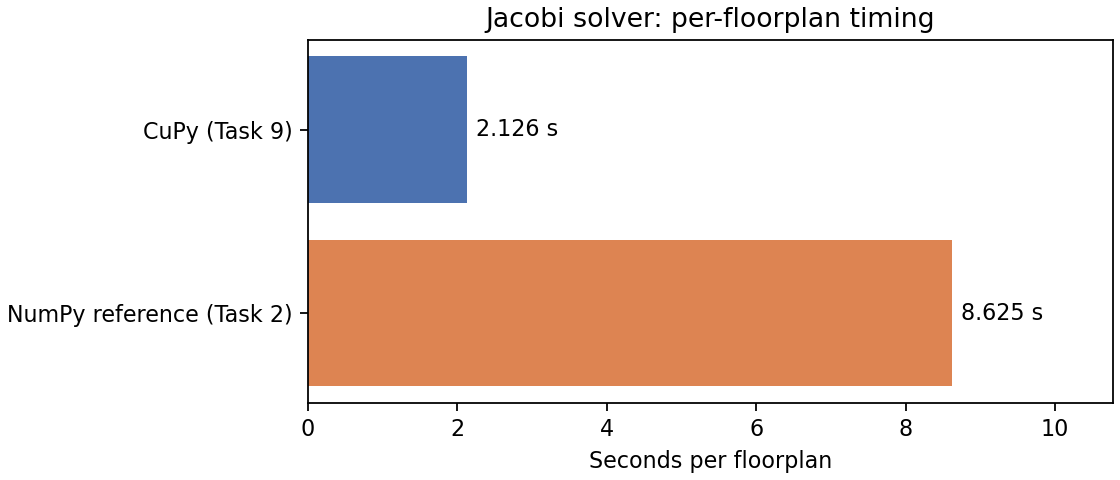
\includegraphics[width=0.7\linewidth]{task9_timing_comparison.png}
    \caption{Per-floor-plan timing of the CuPy solver versus the NumPy
    reference.}
    \label{fig:task9-timing}
\end{figure}

The relatively large warmup overhead (\(\approx \SI{5.1}{\second}\)) is CuPy
compiling its built-in GPU kernels on first use; the relevant figure is the
post-warmup throughput.

\subsection*{9b) Estimate for the full dataset}

\[
    2.126 \text{ s} \times 4571 \approx 9{,}718 \text{ s} \approx 162.0 \text{ min} \approx 2.7 \text{ h}.
\]

\subsection*{9c) Surprising performance observation}

The CuPy port is only \(4.1\times\) faster than the NumPy reference, much
slower than the custom Numba CUDA kernel (\(10.5\times\), Task~8) on the
\emph{same} GPU, and even slower than a 64-core CPU run with dynamic scheduling
(\(19.65\times\), Task~6). This was surprising given that CuPy delegates all
array operations to highly optimised cuBLAS/cuDNN kernels.

The bottleneck is the per-iteration convergence check:

\begin{lstlisting}
delta = float(cp.abs(u_new[mask_gpu] - u_gpu[1:-1, 1:-1][mask_gpu]).max())
\end{lstlisting}

The \texttt{float(\,\dots\,)} call transfers a single scalar from GPU memory
back to the CPU, which forces a \textbf{GPU\(\rightarrow\)CPU
synchronisation} on every iteration. With up to 20{,}000 iterations per floor
plan this produces tens of thousands of pipeline stalls per building. The
actual GPU arithmetic is fast; the synchronisation overhead dominates. Task~10
diagnoses this with \texttt{nsys} and fixes it by batching the convergence
check.

% =====================================================================
\section{Task 10 -- Profiling CuPy with \texttt{nsys} and fixing the issue}
% =====================================================================

The CuPy solver was profiled with NVIDIA's \texttt{nsys} on a single building:

\begin{lstlisting}[language=bash]
nsys profile --output nsys_original python simulate_cupy.py 1 <data_dir>
nsys stats nsys_original.nsys-rep
\end{lstlisting}

The relevant section of the report is the \emph{CUDA API Summary
(cudaapisum)}. For the original CuPy solver it showed
\texttt{cuMemcpyDtoH\_v2} (Device\(\rightarrow\)Host copy) being called
thousands of times (one per Jacobi iteration) and accounting for
\(\approx 95\%\) of total CUDA-API time. In contrast, the simple double-kernel
example from the week 10 lecture only had two such calls. Each
\texttt{cuMemcpyDtoH\_v2} forces CuPy to flush all pending GPU work before
copying the scalar to host memory: a full pipeline stall per iteration.

\subsection*{Fix: batched convergence check}

Only perform the GPU\(\rightarrow\)CPU transfer every
\texttt{CHECK\_INTERVAL = 100} iterations, reducing the number of syncs from
up to 20{,}000 down to \(\approx 200\) per building:

\begin{lstlisting}
if i % check_interval == check_interval - 1:
    delta = float(cp.abs(u_new[mask_gpu] - u_gpu[1:-1, 1:-1][mask_gpu]).max())
    converged = delta < atol
else:
    converged = False

u_gpu[1:-1, 1:-1] = cp.where(mask_gpu, u_new, u_gpu[1:-1, 1:-1])

if converged:
    break
\end{lstlisting}

\(\delta\) is computed \emph{before} the in-place update of \texttt{u\_gpu}, so
the convergence semantics match the original (the only side effect is that we
may run up to 99 extra iterations past convergence, which is negligible).
Re-profiling the optimised version with \texttt{nsys} confirms the diagnosis:
\texttt{cuMemcpyDtoH\_v2} now appears only \(\approx 100\) times and
\texttt{cuLaunchKernel} dominates instead, which is the healthy profile we
expect for a GPU-bound stencil computation.

\subsection*{Timing results}

\begin{table}[H]
    \centering
    \begin{tabular}{lrr}
        \toprule
        Variant                   & Per-floor-plan \([s]\) & Speed-up vs Task~9 \\
        \midrule
        CuPy original (Task~9)    & 2.126 & \(1.00\times\) \\
        CuPy optimised (Task~10)  & 0.828 & \(\mathbf{2.57\times}\) \\
        Numba CUDA (Task~8)       & 0.821 & --- \\
        \bottomrule
    \end{tabular}
    \caption{Effect of the batched convergence check (\(N = 10\) floor plans
    on an A100 GPU).}
    \label{tab:task10-timing}
\end{table}

\begin{figure}[H]
    \centering
    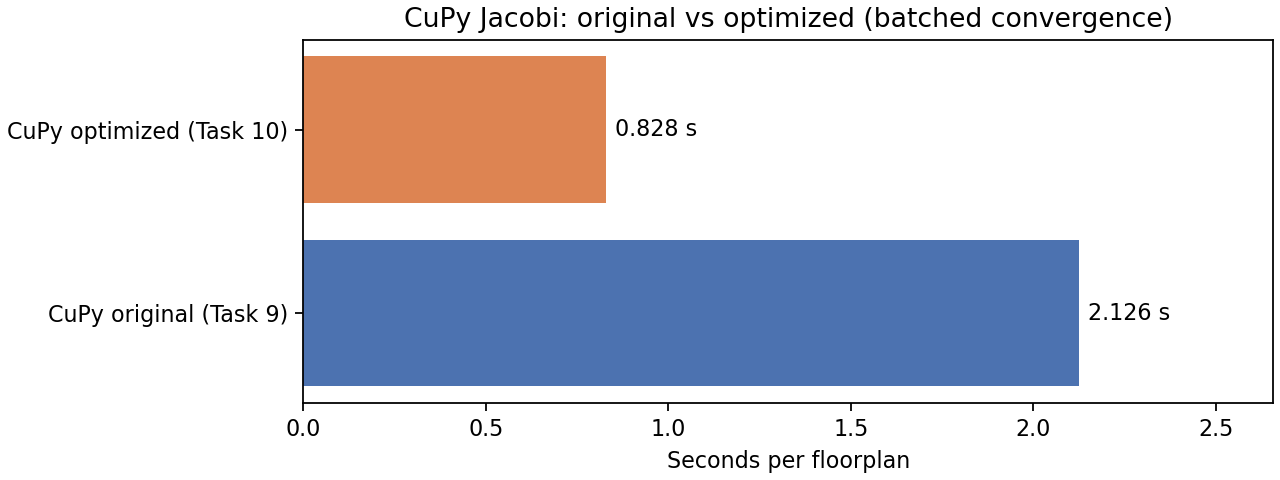
\includegraphics[width=0.7\linewidth]{task10_timing_comparison.png}
    \caption{Per-floor-plan timing of the original (Task~9) versus optimised
    (Task~10) CuPy solver.}
    \label{fig:task10-timing}
\end{figure}

The optimised CuPy is \(\mathbf{2.57\times}\) faster than the original and
matches the hand-written Numba CUDA kernel almost exactly
(\SI{0.828}{\second} vs \SI{0.821}{\second}). This confirms that the
high-level CuPy array API is competitive with a custom CUDA kernel for this
workload, once the per-iteration synchronisation is removed.

\subsection*{Estimate for the full dataset (optimised)}

\[
    0.828 \text{ s} \times 4571 \approx 3{,}785 \text{ s} \approx 63.1 \text{ min}.
\]

\noindent\emph{Note:} mean temperatures from the optimised version differ very
slightly from the original (e.g.\ 14.0131 vs 14.0123 for building 10000)
because the batched check may run up to 99 extra iterations past convergence,
marginally refining the solution. The deviation is well below the practical
accuracy of the simulation.

% =====================================================================
\section{Task 12 -- Full dataset analysis}
% =====================================================================

All 4571 buildings were processed with the optimised CuPy solver from Task~10.
The per-building summary statistics were written to
\texttt{outputs/12-full-analysis/all\_results.csv} and analysed with Pandas in
\texttt{src/12-full-analysis/analyze\_results.py}.

\subsection*{12a) Distribution of mean temperatures}

Figure~\ref{fig:task12-histograms} shows the four distributions of interest
(mean temperature, temperature standard deviation, percentage of area above
18\,\textdegree C and percentage of area below 15\,\textdegree C), one
histogram per building characteristic. The distribution of the mean interior
temperature is centred around 14--15\,\textdegree C with a long left tail of
poorly heated buildings. Buildings with many hot inside walls cluster towards
the higher end; buildings dominated by cold load-bearing walls cluster at the
lower end.

\begin{figure}[H]
    \centering
    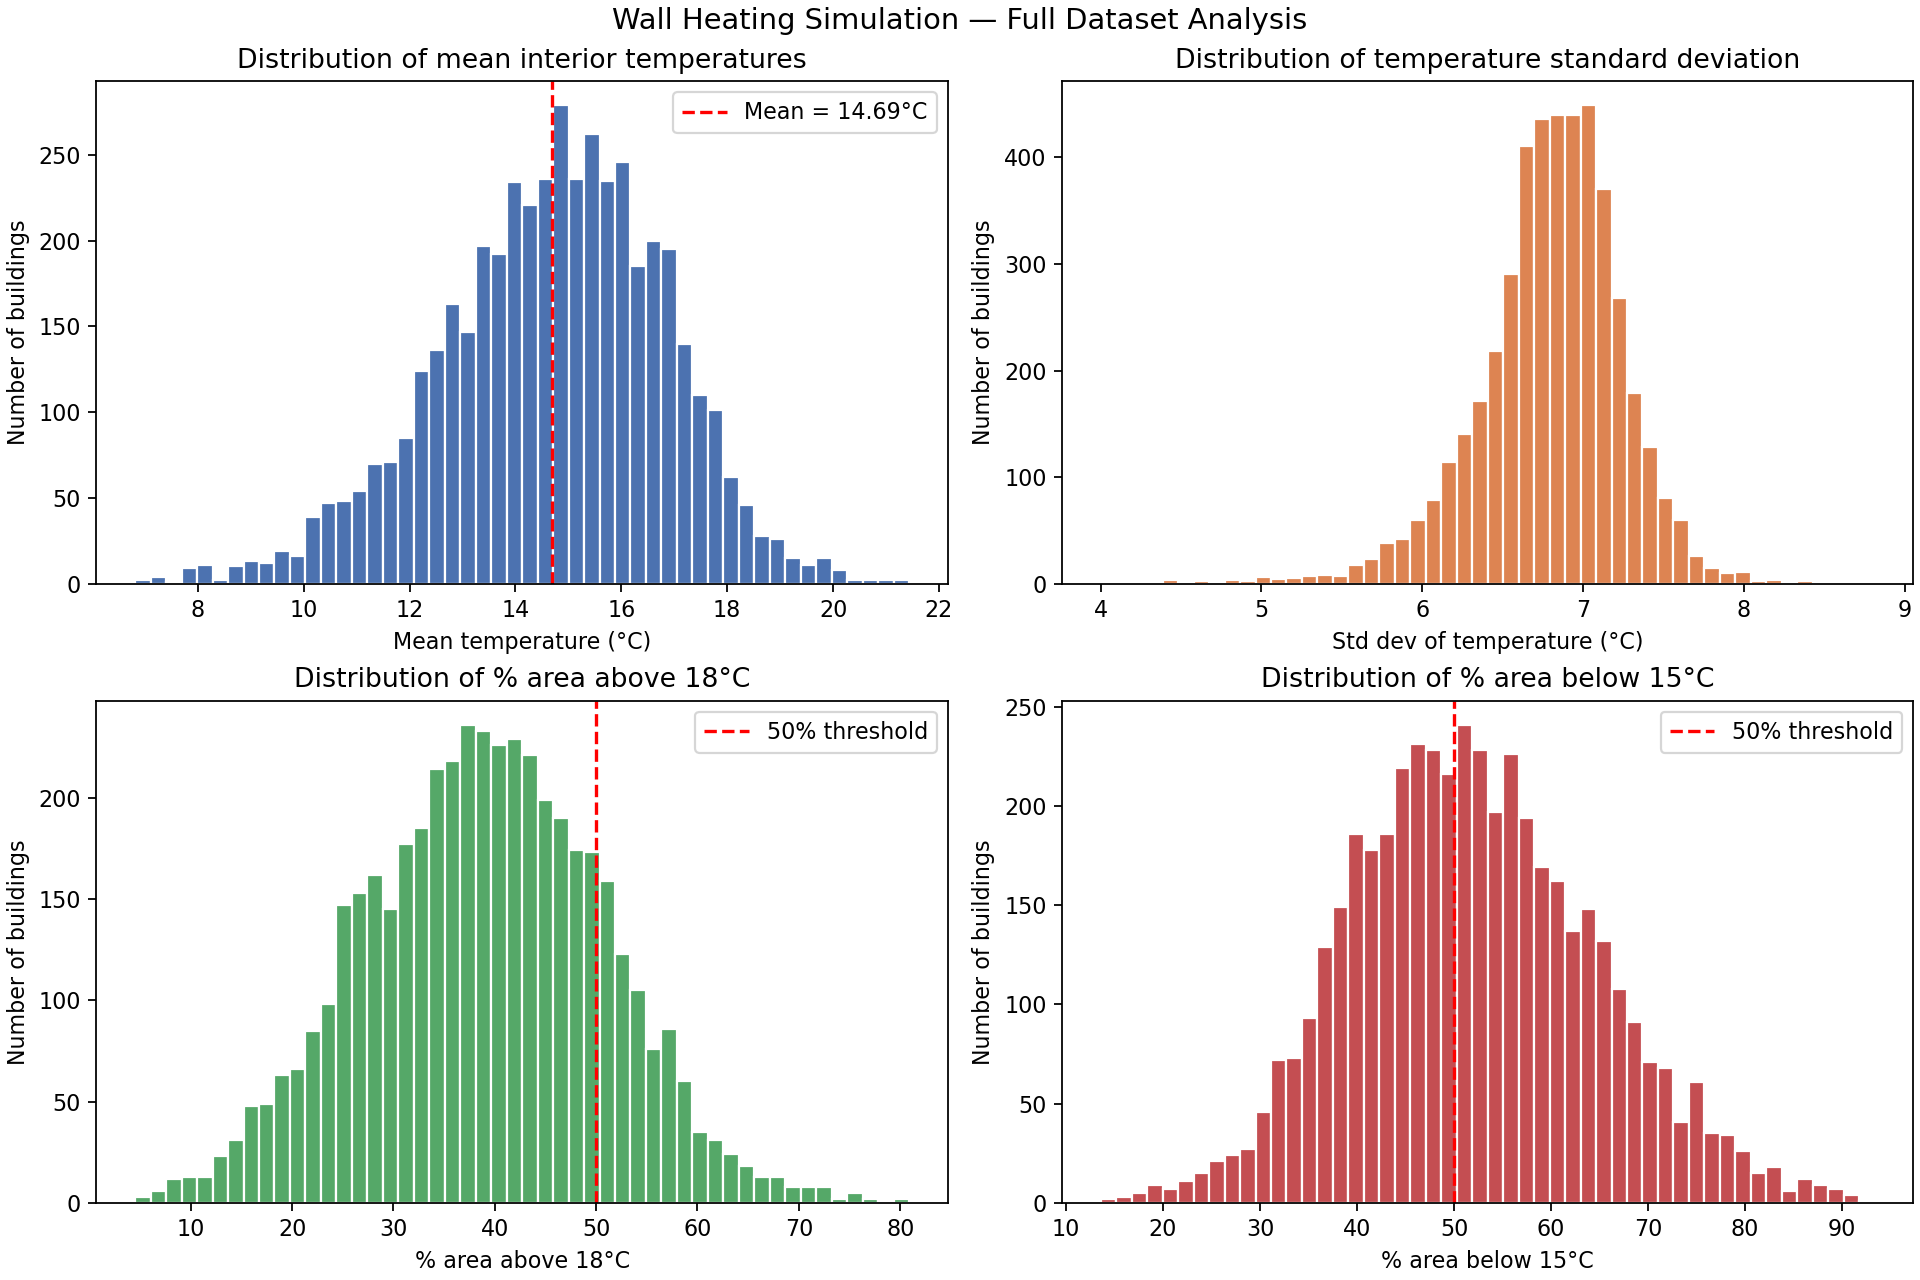
\includegraphics[width=0.95\linewidth]{task12_histograms.png}
    \caption{Distributions of the four per-building summary statistics over
    all 4571 floor plans (top-left: mean temperature; top-right: temperature
    standard deviation; bottom-left: \% area above 18\,\textdegree C;
    bottom-right: \% area below 15\,\textdegree C). The dashed vertical line
    in the bottom panels marks the 50\,\% threshold used in 12d) and 12e).}
    \label{fig:task12-histograms}
\end{figure}

\subsection*{12b) Average mean temperature}

\[
    \overline{\mu_T} = 14.6942\;\text{\textdegree C}
\]

\subsection*{12c) Average temperature standard deviation}

\[
    \overline{\sigma_T} = 6.8016\;\text{\textdegree C}
\]

A larger standard deviation indicates more uneven heating: hot spots near
inside walls combined with cold spots near load-bearing walls.

\subsection*{12d) Buildings with at least 50\,\% area above 18\,\textdegree C}

\[
    n_{>18} = 804 \;/\; 4571 \approx 17.6\%.
\]

These are the well-heated buildings. The Wall Heating approach is most
effective in floor plans with extensive inside-wall coverage relative to floor
area.

\subsection*{12e) Buildings with at least 50\,\% area below 15\,\textdegree C}

\[
    n_{<15} = 2471 \;/\; 4571 \approx 54.1\%.
\]

More than half of the dataset has the majority of its interior at
uncomfortably cold temperatures. These are typically buildings with few inside
walls (most walls are load-bearing) or with large open rooms whose centres are
far from any heated wall.

\subsection*{Verdict on Wall Heating}

Across the full dataset, Wall Heating only manages to keep at least half of
the interior above 18\,\textdegree C in about one in six buildings, while more
than half of the buildings end up with the majority of their area below
15\,\textdegree C. With load-bearing walls fixed at 5\,\textdegree C, the
heated inside walls simply cannot push enough energy through the rooms to
overcome the cold boundary, especially in floor plans with large open spaces
or sparse inside-wall coverage. As an experimental retrofit replacing
radiators, Wall Heating in its current form is therefore not a viable solution
for most of the buildings in the Modified Swiss Dwellings dataset.

% =====================================================================
\section*{Summary of optimisations}
% =====================================================================

Table~\ref{tab:summary} consolidates the per-floor-plan timing of every
solution and the corresponding estimate for the full dataset of 4571
buildings.

\begin{table}[H]
    \centering
    \begin{tabular}{lrrr}
        \toprule
        Solution & Per-floor-plan \([s]\) & Speed-up vs ref. & Full dataset \\
        \midrule
        Reference NumPy (Task 2)              & 8.625 & \(1.0\times\)  & 10.95 h \\
        Numba JIT, single CPU core (Task 7)   & 3.643 & \(2.4\times\)  & 4.6 h \\
        Static scheduling, 64 cores (Task 5)  & 0.432 & \(20.0\times\) & 32.9 min \\
        Dynamic scheduling, 64 cores (Task 6) & 0.374 & \(23.1\times\) & 28.5 min \\
        CuPy reference port (Task 9)          & 2.126 & \(4.1\times\)  & 162.0 min \\
        Numba CUDA kernel (Task 8)            & 0.821 & \(10.5\times\) & 62.6 min \\
        CuPy optimised, batched check (Task 10) & 0.828 & \(10.4\times\) & 63.1 min \\
        \bottomrule
    \end{tabular}
    \caption{Per-floor-plan timing and full-dataset estimate for every
    implementation explored in this project.}
    \label{tab:summary}
\end{table}

\noindent The dynamic-scheduling CPU solution remains the fastest end-to-end
configuration overall thanks to its 64-fold parallelism, while the optimised
CuPy and Numba CUDA kernels deliver the best single-device throughput and only
need a single GPU to bring the full dataset down to about an hour.

\end{document}
